\documentclass[10pt,twocolumn]{article}

\usepackage[a4paper,margin=2cm]{geometry}
\usepackage[T1]{fontenc}
\usepackage{lmodern}
\usepackage[colorlinks,urlcolor=blue,linkcolor=blue,citecolor=blue]{hyperref}
\hypersetup{
  pdftitle={A Functional Taxonomy of the Web of Agents: Operational Definitions and an Empirical Validation Protocol},
  pdfauthor={Tatiana Petrova},
  pdfsubject={Web of Agents, multi-agent systems, LLM interoperability taxonomy},
  pdfkeywords={Web of Agents, multi-agent systems, large language models, agent interoperability, Model Context Protocol, taxonomy, inter-rater reliability},
  pdflang={en}
}
\usepackage{graphicx}
\graphicspath{{figures/}{./}}
\usepackage{amsmath,amsfonts,amssymb}
\usepackage{array}
\usepackage{textcomp}
\usepackage{url}
\usepackage[numbers,sort&compress]{natbib}
\usepackage{tikz}
\usetikzlibrary{arrows.meta, positioning, shapes.geometric}
\usepackage{xcolor}
\usepackage{tabularx}
\newcolumntype{Y}{>{\raggedright\arraybackslash}X}
\usepackage{booktabs}
\usepackage{caption}
\usepackage{authblk}

\setlength{\parindent}{1em}

\title{A Functional Taxonomy of the Web of Agents: Operational Definitions and an Empirical Validation Protocol}

\author[1]{Tatiana Petrova}
\affil[1]{University of Luxembourg}

\date{April 2026}

\begin{document}

\twocolumn[
\begin{@twocolumnfalse}
\maketitle
\begin{abstract}
The ``Web of Agents'' (WoA) has cycled through three architectural generations, FIPA/BDI multi-agent systems, the Semantic Web, and LLM-powered agents, with markedly different adoption outcomes.  Existing taxonomies describe these generations chronologically but offer neither operational classification criteria nor empirical validation.  We contribute a four-axis functional taxonomy (semantic foundation, communication paradigm, locus of intelligence, discovery mechanism) together with (i)~an operational codebook specifying measurable criteria for each axis-value, (ii)~a pre-registered three-part validation protocol covering inter-rater reliability, predictive validity, and LLM-based classification, and (iii)~a three-rater LLM-self-consistency pilot on five systems against a locally archived corpus, yielding a mean pairwise Cohen's $\kappa$ of $\{1.00, 0.81, 0.80, 1.00\}$ across the four axes.  Item-level disagreements are attributable to genuine corpus silence rather than classifier divergence.  The taxonomy yields a testable hypothesis, that adoption correlates with \emph{axis coherence} rather than with any single axis value, which reframes the familiar ``paradigm shift'' narrative as an empirical claim rather than a post-hoc explanation.  No quantitative conclusions about that hypothesis are drawn here; we specify the data and the decision rule under which it would be supported or falsified by the planned full execution with human coders.
\end{abstract}
\vspace{1em}
\end{@twocolumnfalse}
]

\textbf{Keywords:} Web of Agents; multi-agent systems; large language models; agent interoperability; Model Context Protocol; agent commerce; AI governance.


%%====================================================================
%% SECTION 1: INTRODUCTION
%%====================================================================
\section{Introduction}

The Web of Agents (WoA) envisions an Internet populated by autonomous software agents that discover one another, communicate through open protocols, and execute tasks on behalf of users, turning the static ``web of documents'' into an environment for machine-to-machine cooperation~\cite{Berners-Lee_2001}. This idea has recurred across three decades, through the Semantic Web era, the Multi-Agent Systems (MAS) community, and the recent wave of Large Language Model (LLM)-powered agents, yet it remained largely aspirational until now.

Three developments have brought the WoA closer to practicability.  Frontier LLMs now provide the general-purpose reasoning that individual agents lacked in earlier generations~\cite{Brown_2020}.  Lightweight open protocols, namely the Model Context Protocol (MCP) for tool access~\cite{MCP_2025} and the Agent-to-Agent (A2A) protocol for inter-agent coordination~\cite{Google_2025_A2A}, build on familiar web primitives (HTTP, JSON-RPC).  And an institutional context has begun to form around these protocols: stewardship transitions to neutral foundations~\cite{AAIF_2025, A2A_LinuxFoundation_2025}, regulatory frameworks~\cite{EUAI_2024}, and industry announcements of agent-commerce infrastructure from payment networks~\cite{Visa_TAP_2025, Mastercard_AgentPay_2025, Stripe_OpenAI_ACP_2025}.  We cite these developments as primary sources that the reader can inspect directly; we do not attempt to summarize their present status, because those details change between the time of writing and the time of reading.

\textbf{Thesis.}  We argue that the WoA has reached a point where the principal bottleneck has moved from \emph{agent capability} (largely addressed by LLMs, despite their known limitations) to \emph{ecosystem infrastructure}: the protocols, identity frameworks, economic models, and governance structures needed to turn isolated agent demos into a functioning internet-scale system.

\textbf{Contributions.}  This article makes three contributions.  First, it \emph{operationalizes} a four-axis functional taxonomy (semantic foundation, communication paradigm, locus of intelligence, discovery mechanism) by supplying measurable criteria for each axis-value in a codebook suitable for third-party coding.  Second, it advances a pre-registered three-part validation protocol (inter-rater reliability, predictive validity on adoption outcomes, LLM-as-classifier agreement) and reports a pilot on five representative systems.  Third, it formulates the ``paradigm shift'' narrative as a falsifiable \emph{axis-coherence hypothesis}, that adoption correlates with alignment across axes rather than with axis values, and specifies the outcomes under which the hypothesis would be rejected.

\textbf{Relation to prior work.}  Recent taxonomies classify agent protocols along technical dimensions (e.g., feature tables comparing MCP, A2A, ACP, ANP).  None, to our knowledge, report inter-rater reliability for their axis assignments, or link taxonomic position to measurable adoption outcomes.  The present article differs in these two respects.


%%====================================================================
%% SECTION 2: THE PARADIGM SHIFT
%%====================================================================
\section{The Paradigm Shift}\label{sec:paradigm}

\subsection{Three Prior Generations and Why Each Failed}

The WoA vision has evolved through three distinct generations, each built on a different architectural bet and each failing for a different reason.

\textbf{Generations 1--2: From Reactive Agents to the FIPA Era (1990--2005).}  The first generation (early 1990s) comprised single-purpose, reactive agents with fixed logic. The BDI architecture~\cite{Rao_1995} formalized deliberative reasoning, but interoperability was ad hoc.  The second generation relied on FIPA, whose Agent Communication Language (ACL), grounded in speech-act theory, offered high semantic expressiveness~\cite{FIPA_2002, Poslad_2007}. FIPA defined a complete platform architecture with centralized coordination, and JADE gained industry traction. Yet FIPA did not take hold at web scale: the formal semantics were too heavy for typical web applications, the architecture was mismatched with the Web's stateless design, and the Agentcities experiment showed that even standards-compliant agents required further agreements to interoperate~\cite{Ciortea_2019}. The result was \emph{vertical success but horizontal failure}: JADE thrived in telecommunications and logistics but not on the open Web, a pattern the Semantic Web later repeated.

\textbf{Generation 3: The Semantic Web Vision (2001--2012).}  Tim Berners-Lee's 2001 scenario~\cite{Berners-Lee_2001} imagined personal agents scheduling medical appointments by reasoning over knowledge graphs built on the Resource Description Framework (RDF) and Web Ontology Language (OWL). The vision foundered on an incentive failure: creating and maintaining large-scale semantic annotations was prohibitively expensive, and no viable economic model justified the effort. The intervening decade produced steady standards work (OWL~1.0 in 2004, SPARQL in 2008, the Linked Data initiative), but none of it resolved this core incentive problem. The gap between 2001 and Schema.org's pragmatic compromise in 2011 (Figure~\ref{fig:history}) reflects a period of diminishing ambition rather than inactivity. Separately, logical inference engines could not cope with the Web's noise, contradiction, and incompleteness. By the mid-2000s, the community acknowledged that the universal agent vision remained largely unrealized~\cite{Hogan_2020}.

The Semantic Web \emph{technology stack}, however, did not fail entirely. Schema.org annotations became widely adopted on the public web, with reported coverage statistics documented by Guha et al.~\cite{Guha_2016}; Knowledge Graphs power search and recommendation at major providers, and RDF-based ontologies (SNOMED-CT, Gene Ontology) underpin biomedical interoperability. What failed was the \emph{universal agent vision}: the expectation that the open Web would adopt rich formal annotations at sufficient scale to support autonomous agent reasoning. This repeated the FIPA-era pattern of vertical success but horizontal failure: today's agent protocols may follow a similar trajectory, gaining traction in specific verticals long before, and possibly instead of, becoming universal. The Semantic Web experience shows that encoding intelligence in external data demands a semantic infrastructure whose cost the open Web cannot justify at universal scale, even though domain-specific deployments remain highly valuable.  Across both generations, the primary bottleneck was not the network but the \emph{nodes}: individual agents lacked the general-purpose reasoning that would have driven adoption of complex interoperability standards. The protocols were ahead of the agents.

\subsection{What LLMs Changed: The Implicit Semantics Shift}

LLMs have moved the locus of semantic understanding from external structures to the agent's internal model, largely closing this gap. A Semantic Web agent required pre-existing RDF/OWL annotations; an LLM-powered agent interprets natural language descriptions, API documentation, and unstructured web content without prior annotation~\cite{Yao_2023, Schick_2023}. FIPA agents needed formal ontologies for mutual understanding. Modern agents achieve pragmatic interoperability through shared natural language and lightweight JSON schemas.

We call this transition the move from ``Semantics in Data'' to ``Semantics in Models.''  The framing resonates with established distinctions but deliberately simplifies a continuum. Modern systems combine implicit understanding with explicit structured metadata (Agent Cards, typed tool schemas), and Retrieval-Augmented Generation (RAG) architectures blur the boundary by injecting external data at inference time; category-aware hybrid retrieval~\cite{Petrova_CARRAG_2025} illustrates how the retrieval layer is now engineered against the LLM's specific failure modes, in that case against hallucination. The distinction is useful insofar as it identifies the \emph{primary locus of semantic engineering effort}, not a binary divide. Within that caveat, three practical consequences stand out.  \emph{Lower integration cost}: new tools can be integrated via natural language descriptions rather than formal ontologies.  \emph{Graceful degradation}: LLM-based understanding degrades smoothly under ambiguity.  \emph{Protocol simplification}: because the agent handles semantic interpretation, the protocol layer can be thin (JSON-RPC over HTTP suffices).

``Semantics in Models'' has its own failure modes. LLMs hallucinate, producing plausible but incorrect outputs without a built-in mechanism for signaling uncertainty. Multi-step reasoning degrades over long chains, and performance is sensitive to prompt phrasing in ways that are hard to audit. Inference costs remain high, and multi-agent workflows can consume orders of magnitude more compute than hand-coded pipelines. For interoperability, the chief limitation is that implicit semantics are \emph{non-verifiable}: unlike a formal ontology, an LLM's interpretation of a tool description cannot be validated prior to execution. The shift holds despite these failure modes, which define the concrete problems for the next wave of protocol and systems work.

\subsection{The 2025--2026 Institutional Convergence}\label{sec:convergence}

Figure~\ref{fig:history} shows the paradigm trajectory. The institutional developments below represent its latest phase.

\textbf{Standards consolidation.}  The principal inter-agent protocols (MCP, A2A, and the earlier ACP) have been, per the cited primary sources, transitioned towards neutral stewardship~\cite{AAIF_2025, A2A_LinuxFoundation_2025, ACP_Merger_2025}.  We take no position on the exact calendar of announcements; what matters for the taxonomy is the structural possibility that governance of Axis-1 descriptors (capability manifests, Agent Cards) may come to reside outside any single vendor, a falsifiable expectation against which the reader can check the state of the ecosystem at any later date.

\textbf{Regulatory pressure.}  The EU AI Act~\cite{EUAI_2024} introduces phased obligations on AI systems including transparency and oversight requirements of direct relevance to multi-agent deployments; NIST's AI Risk Management Framework~\cite{NIST_AI_600_2024} and the International AI Safety Report~\cite{AISAFETY_2025} frame the associated risks.  Specific enforcement dates and sectoral scope evolve between versions of these documents; we cite the primary sources rather than reproduce timelines here.

\textbf{Commercial momentum.}  Announcements from major payment networks signal emerging interest in agent-mediated commerce~\cite{Visa_TAP_2025, Mastercard_AgentPay_2025, Stripe_OpenAI_ACP_2025}; we forward the reader to the cited primary sources rather than summarize product scope, which is likely to change.  What matters for the taxonomy is that an economic layer, largely absent from prior generations, is now at least being proposed.

\begin{figure*}[!t]
\centering
\resizebox{\textwidth}{!}{%
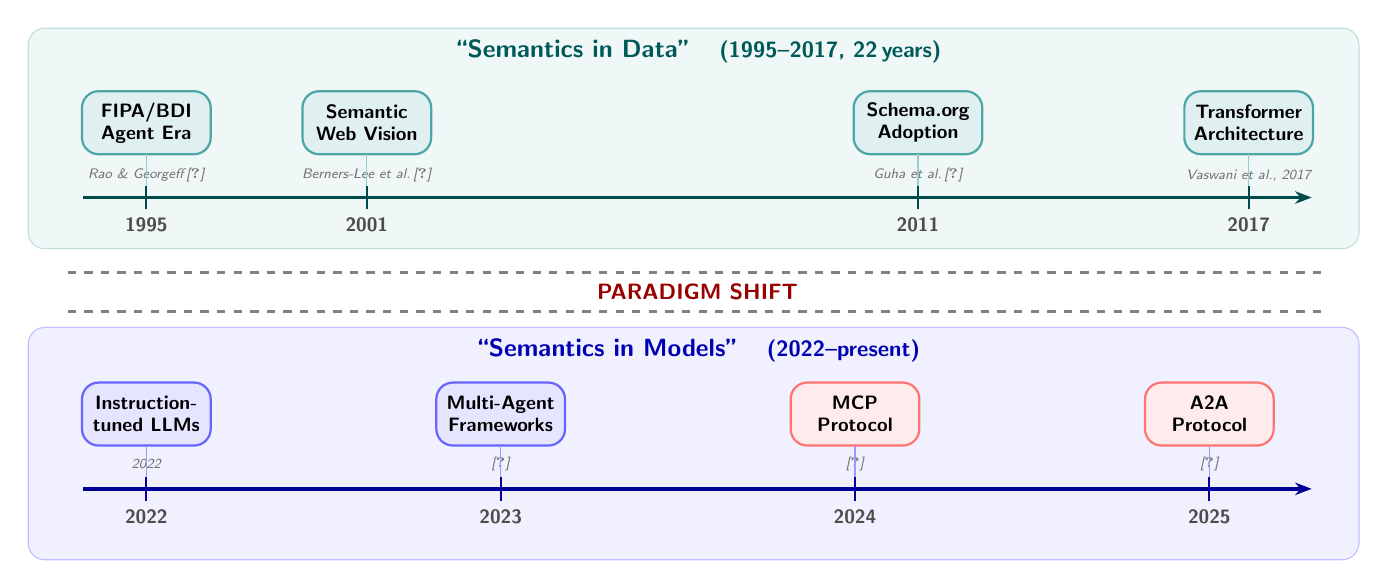
\begin{tikzpicture}[
    >=Stealth,
    databox/.style={rectangle, rounded corners=6pt, draw=teal!70, thick,
                fill=teal!12, text width=1.4cm, minimum height=0.8cm,
                font=\sffamily\scriptsize\bfseries, align=center, text=black},
    modelbox/.style={rectangle, rounded corners=6pt, draw=blue!60, thick,
                fill=blue!10, text width=1.4cm, minimum height=0.8cm,
                font=\sffamily\scriptsize\bfseries, align=center, text=black},
    protobox/.style={rectangle, rounded corners=6pt, draw=red!55, thick,
                fill=red!8, text width=1.4cm, minimum height=0.8cm,
                font=\sffamily\scriptsize\bfseries, align=center, text=black},
    yearlbl/.style={font=\sffamily\scriptsize\bfseries, text=black!70},
    eralbl/.style={font=\sffamily\small\bfseries},
    attrib/.style={font=\sffamily\tiny\itshape, text=black!55},
]
\fill[teal!6, rounded corners=6pt, draw=teal!25, thin] (-1.5, 2.55) rectangle (15.4, 5.35);
\node[eralbl, text=teal!70!black] at (7.0, 5.05)
    {\textbf{``Semantics in Data''}\quad{\footnotesize(1995--2017, 22\,years)}};
\draw[-{Stealth[length=6pt]}, line width=1.2pt, teal!60!black]
    (-0.8, 3.2) -- (14.8, 3.2);
\foreach \x in {0, 2.8, 9.8, 14.0}
    \draw[teal!60!black, thick] (\x, 3.05) -- (\x, 3.35);
\node[yearlbl] at (0, 2.85)    {1995};
\node[yearlbl] at (2.8, 2.85)  {2001};
\node[yearlbl] at (9.8, 2.85)  {2011};
\node[yearlbl] at (14.0, 2.85) {2017};
\node[databox]  at (0, 4.15)    {FIPA/BDI\\Agent Era};
\node[attrib]   at (0, 3.48)    {Rao \& Georgeff\,\cite{Rao_1995}};
\node[databox]  at (2.8, 4.15)  {Semantic\\Web Vision};
\node[attrib]   at (2.8, 3.48)  {Berners-Lee et al.\,\cite{Berners-Lee_2001}};
\node[databox]  at (9.8, 4.15)  {Schema.org\\Adoption};
\node[attrib]   at (9.8, 3.48)  {Guha et al.\,\cite{Guha_2016}};
\node[databox]  at (14.0, 4.15) {Transformer\\Architecture};
\node[attrib]   at (14.0, 3.48) {Vaswani et al., 2017};
\foreach \x in {0, 2.8, 9.8, 14.0}
    \draw[teal!40, thin] (\x, 3.35) -- (\x, 3.75);
\draw[dashed, black!50, line width=1pt] (-1.0, 2.25) -- (15.0, 2.25);
\node[font=\sffamily\footnotesize\bfseries, text=red!60!black,
      fill=white, inner xsep=6pt, inner ysep=2pt, rounded corners=2pt]
    at (7.0, 2.0) {PARADIGM SHIFT};
\draw[dashed, black!50, line width=1pt] (-1.0, 1.75) -- (15.0, 1.75);
\fill[blue!6, rounded corners=6pt, draw=blue!25, thin] (-1.5, -1.4) rectangle (15.4, 1.55);
\node[eralbl, text=blue!70!black] at (7.0, 1.25)
    {\textbf{``Semantics in Models''}\quad{\footnotesize(2022--present)}};
\draw[-{Stealth[length=6pt]}, line width=1.2pt, blue!60!black]
    (-0.8, -0.5) -- (14.8, -0.5);
\foreach \x in {0, 4.5, 9.0, 13.5}
    \draw[blue!60!black, thick] (\x, -0.65) -- (\x, -0.35);
\node[yearlbl] at (0, -0.85)    {2022};
\node[yearlbl] at (4.5, -0.85)  {2023};
\node[yearlbl] at (9.0, -0.85)  {2024};
\node[yearlbl] at (13.5, -0.85) {2025};
\node[modelbox]  at (0, 0.45)     {Instruction-\\tuned LLMs};
\node[attrib]    at (0, -0.18)    {2022};
\node[modelbox]  at (4.5, 0.45)   {Multi-Agent\\Frameworks};
\node[attrib]    at (4.5, -0.18)  {\cite{Microsoft_AutoGen_2023}};
\node[protobox]  at (9.0, 0.45)   {MCP\\Protocol};
\node[attrib]    at (9.0, -0.18)  {\cite{MCP_2025}};
\node[protobox]  at (13.5, 0.45)  {A2A\\Protocol};
\node[attrib]    at (13.5, -0.18) {\cite{Google_2025_A2A}};
\foreach \x in {0, 4.5, 9.0, 13.5}
    \draw[blue!40, thin] (\x, -0.35) -- (\x, 0.05);
\end{tikzpicture}%
}%
\caption{\textbf{The evolutionary paradigm shift from ``Semantics in Data'' to ``Semantics in Models.''}
``Semantics in Data'' (top row) denotes architectures where shared meaning is encoded in external structures (ontologies, RDF/OWL schemas, annotated knowledge graphs). ``Semantics in Models'' (bottom row) denotes architectures where meaning is implicitly captured in LLM representations. Both rows span the same width but cover different periods: the pre-LLM era produced four major milestones over two decades, whereas the post-Transformer era matched that count in under three years, illustrating the pace of change.}
\label{fig:history}
\end{figure*}


%%====================================================================
%% SECTION 3: FUNCTIONAL TAXONOMY
%%====================================================================
\section{Functional Taxonomy}\label{sec:taxonomy}

A chronological narrative, however useful, does not by itself explain \emph{why} successive generations failed differently. We therefore introduce a four-axis functional taxonomy (Figure~\ref{fig:taxonomy}) designed to compare WoA architectures from any era along the dimensions most relevant to interoperability.

\subsection{Derivation and Scope}

We derive the four axes from the four interoperability-facing decisions that every agent architecture must make explicitly or by default: how to represent shared meaning, how to structure a message, where to place inference, and how to locate peers.  Prior generational retrospectives~\cite{Ciortea_2019, Hogan_2020} identify each of these decisions, but as separate narratives rather than as orthogonal dimensions of a single design space.

The taxonomy is deliberately limited to interoperability-facing properties; intra-agent dimensions (autonomy level, planning paradigm, world-model richness) are excluded because they describe what happens \emph{inside} an agent rather than \emph{between} agents.  Trust, security, and compliance cross-cut all four axes and are treated as research challenges (Section~\ref{sec:frontier}) rather than as further axes, pending a stable design space.

\subsection{Four Axes of Classification}

Each axis is defined below together with an \emph{observable} criterion that a coder can apply to a system's public specification and reference implementation.  Full operational definitions, tie-breaking rules, and worked examples are given in the accompanying codebook (Supplementary Material, \textsection\,A1--A4).  Values are ordered on a \emph{structured} to \emph{flexible} spectrum and reported as $\{0.0, 0.5, 1.0\}$ for analysis (Section~\ref{sec:validation}).

\textbf{Axis 1: Semantic Foundation.}  Where is shared meaning represented at exchange time?
\emph{0.0 Formal}, the specification requires conformance to an explicit ontology (RDF, OWL, SHACL);
\emph{0.5 Procedural}, messages carry an enumerated performative whose semantics are fixed by the communication-language specification (FIPA ACL);
\emph{1.0 Implicit}, capabilities are described in unstructured natural language that an LLM interprets at call time, with structural (non-ontological) JSON Schema at most.

\textbf{Axis 2: Communication Paradigm.}  What is the primary abstraction of a message?
\emph{0.0 Performative}, illocutionary acts from a finite vocabulary with defined interaction protocols;
\emph{0.5 Resource-oriented}, operations on URI-identified resources with hypermedia-driven state transitions;
\emph{1.0 RPC-style}, named procedure invocations with typed arguments (JSON-RPC, gRPC).

\textbf{Axis 3: Locus of Intelligence.}  Which component performs non-trivial inference at task time?
\emph{0.0 Data}, reasoning is performed by rule engines over annotated knowledge graphs;
\emph{0.5 Platform}, middleware supplies domain-agnostic coordination (directory facilitators, matchmakers, interaction protocols);
\emph{1.0 Agent/Model}, a language model within the agent performs open-ended reasoning; the protocol carries data, not reasoning.

\textbf{Axis 4: Discovery Mechanism.}  How does one agent locate a peer providing a required capability?
\emph{0.0 Centralized registry}, a single authoritative index (FIPA DF, UDDI, canonical MCP Registry);
\emph{0.5 Standardized metadata}, capability descriptors at well-known URLs on the provider itself (A2A Agent Cards);
\emph{1.0 Decentralized/networked}, peer-to-peer substrate with no authoritative registry (DID-based, DHT)~\cite{W3C_ANP_2025}.

\textbf{Coherence score.}  For a system $S$ with axis values $(a_1, a_2, a_3, a_4) \in [0,1]^4$ we define $\mathrm{coh}(S) = 1 - 2\cdot\mathrm{std}(a_1, a_2, a_3, a_4)$.  A profile aligned on any one side yields $\mathrm{coh}(S) \approx 1$; a zigzag profile yields $\mathrm{coh}(S) \approx 0$.  The central empirical claim we evaluate is whether $\mathrm{coh}(S)$ is associated with adoption outcomes after controlling for generation and domain (Section~\ref{sec:validation}).

\subsection{Application to Generational Archetypes}

Table~\ref{tab:taxonomy} applies the taxonomy to four generational archetypes, including the emerging post-2025 era.  We distinguish this latest era from the preceding LLM era not by a shift in underlying AI capability but by a qualitative change in ecosystem infrastructure: neutral governance, regulatory frameworks, and commercial payment rails arriving together create a distinct operating context for the same LLM-powered agents.  The date ranges intentionally overlap at 2025.

\begin{table*}[!t]
\centering
\caption{Functional taxonomy and protocol stack across WoA generations}
\label{tab:taxonomy}
\begin{tabularx}{\textwidth}{|l|X|X|X|X|}
\hline
\textbf{Dimension} & \textbf{FIPA-based MAS} & \textbf{Semantic Web Agents} & \textbf{LLM-based (2023--25)} & \textbf{Post-2025 Era$^\dagger$} \\
\hline
\multicolumn{5}{|l|}{\textit{Taxonomy axes}} \\
\hline
\textbf{Semantic Foundation} & Procedural: speech-act semantics~\cite{FIPA_2002} & Formal: ontologies (RDF, OWL)~\cite{Berners-Lee_2001, Hogan_2020} & Implicit: LLM world model~\cite{Brown_2020} & \emph{Hybrid: implicit + structured metadata}~\cite{AAIF_2025, A2A_v03_2025} \\
\hline
\textbf{Communication} & Performative (FIPA ACL)~\cite{FIPA_2002} & Resource-oriented~\cite{Ciortea_2019} & RPC (JSON-RPC)~\cite{MCP_2025, Google_2025_A2A} & RPC + streaming + \emph{negotiation}~\cite{A2A_v03_2025} \\
\hline
\textbf{Locus of Intelligence} & Platform (DF, AMS)~\cite{Poslad_2007} & Data (knowledge graphs)~\cite{Berners-Lee_2001} & Agent/Model (LLM)~\cite{Yao_2023, Schick_2023} & Agent + \emph{federated registries}~\cite{AAIF_2025} \\
\hline
\textbf{Discovery} & Centralized (DF)~\cite{Poslad_2007} & SPARQL endpoints~\cite{Hogan_2020} & Metadata (\texttt{agent.json})~\cite{Google_2025_A2A} & \emph{Hybrid: registries + DIDs}~\cite{AAIF_2025, W3C_ANP_2025} \\
\hline
\multicolumn{5}{|l|}{\textit{Protocol-stack dimensions}} \\
\hline
\textbf{Governance} & FIPA (dissolved 2005)~\cite{Poslad_2007} & W3C standards track & Vendor-led~\cite{MCP_2025, Google_2025_A2A} & Neutral foundations~\cite{AAIF_2025, A2A_LinuxFoundation_2025} \\
\hline
\textbf{Identity \& Auth} & Platform certificates~\cite{Poslad_2007} & URI-based & Ad hoc / OAuth 2.0 & OAuth 2.1 + DIDs + KYA~\cite{MCP_Tasks_2025, W3C_ANP_2025, KYA_Paradigm_2025} \\
\hline
\textbf{Commerce} & Not addressed & Not addressed & Stripe/OpenAI~\cite{Stripe_OpenAI_ACP_2025} & Trusted Agent Protocols~\cite{Visa_TAP_2025, Mastercard_AgentPay_2025} \\
\hline
\textbf{User Interface} & None standardized & Browser-based & Ad hoc & AG-UI (streaming)~\cite{AGUI_2025}; WebMCP~\cite{WebMCP_W3C_2025} \\
\hline
\multicolumn{5}{l}{\footnotesize $^\dagger$\,Italicized entries denote nascent or proposed capabilities, not yet deployed at scale.}
\end{tabularx}
\end{table*}

The post-2025 era keeps the LLM-powered ``intelligence-in-agent'' choice from the prior generation but adds institutional infrastructure (registries, governance, identity, commerce) that earlier generations attempted through purely technical means.  The era does not abandon structured metadata but lowers its ambition, from universal ontologies to lightweight JSON schemas that LLMs can interpret without formal reasoning engines.  Structured metadata remains necessary (Agent Cards, typed tool schemas, capability manifests), but the semantic burden has shifted from the data to the model, confirming that the paradigm boundary is a spectrum rather than a binary.

Each generation failed because of \emph{mismatches between axes} (Figure~\ref{fig:taxonomy}).  Consider the Semantic Web: it offered the richest semantic foundation (Axis~1: formal ontologies) but coupled it with infrastructure-dependent discovery (Axis~4), placed intelligence in external data (Axis~3), and relied on resource-oriented communication (Axis~2) that had no natural mechanism for agent-initiated action.  The result was a system where data was expressive but agents were weak, a mismatch between Axes~1 and~3.  FIPA suffered a complementary mismatch: it had the appropriate intelligence model (Axis~3: platform-mediated reasoning) and expressive communication (Axis~2: speech acts), but its formal semantics (Axis~1) and centralized discovery (Axis~4) were architecturally incompatible with the stateless, decentralized Web.  In Figure~\ref{fig:taxonomy}, these mismatches appear as \emph{zigzag} patterns across axes, whereas the LLM and post-2025 eras cluster on the right side of each spectrum (with the notable exception of LLM-era discovery, which sits at the midpoint).

\textbf{Limitations.}  The taxonomy focuses on \emph{interoperability-facing} properties. Dimensions that characterize individual agents (autonomy level, internal planning paradigm) are excluded because they describe what happens \emph{inside} an agent rather than \emph{between} agents.  Trust cross-cuts all four axes and is therefore treated as a research challenge below. A future refinement might decompose it into a fifth axis once the design space stabilizes.  The post-2025 column in Table~\ref{tab:taxonomy} is partly aspirational, and we stylize our generational archetypes; real systems often blend features across generations (e.g., a JADE-based agent augmented with an LLM reasoning layer).

\begin{figure}[!t]
\centering
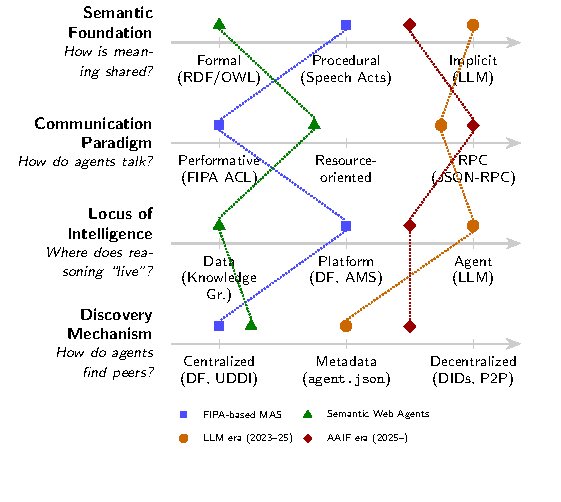
\includegraphics[width=\columnwidth]{fig2_taxonomy.pdf}
\caption{\textbf{Generational profiles across the four taxonomy axes.}  Each axis progresses from more structured, formal approaches (left) to more flexible, emergent ones (right).  Marker positions are the median values assigned by independent coders applying the operational criteria in the supplementary codebook to a reference exemplar of each generation; full coding sheets are released with the supplementary material.  Dotted lines connecting markers of the same generation visualize \emph{axis coherence} (Section~\ref{sec:taxonomy}): the LLM-era exemplar aligns on the right, the Semantic-Web exemplar on the left, and the FIPA-era exemplar exhibits a zigzag pattern.  Whether this pattern correlates with adoption outcomes beyond these four exemplars is the empirical question tested in Section~\ref{sec:validation}.}
\label{fig:taxonomy}
\end{figure}


%%====================================================================
%% SECTION 4: MODERN PROTOCOL STACK
%%====================================================================
\section{Modern Protocol Stack}\label{sec:stack}

\subsection{MCP and A2A: Complementary Roles}\label{sec:mcp-a2a}

MCP and A2A serve complementary roles. MCP standardizes how an agent accesses external tools and data (the ``vertical'' axis), while A2A standardizes how agents communicate with each other (the ``horizontal'' axis)~\cite{MCP_2025, Google_2025_A2A}. Together they form the core of the current agent stack.

\textbf{Example.} A user asks a personal assistant on a car-dealer website to ``find an SUV under \texteuro40\,000 with low mileage and book a test drive.''  The assistant queries the dealer's inventory via MCP, discovers and delegates to an independent financing-and-insurance agent via A2A (obtaining a loan pre-approval, insurance quote, and trade-in valuation), then books a test-drive slot through the dealer's scheduling MCP server.  As Figure~\ref{fig:sequence} illustrates, MCP handles tool invocations against the dealer's own systems while A2A orchestrates cross-organizational delegation, showing the multi-stakeholder coordination that distinguishes the WoA from a single-vendor integration.

Both protocols adopt JSON-RPC rather than REST because agent interactions are action-oriented (``call this function,'' ``run this task''), and JSON-RPC maps directly to LLM tool-calling APIs~\cite{Schick_2023}.  The trade-off is non-trivial: abandoning REST means losing HATEOAS (Hypermedia as the Engine of Application State), through which a REST client can discover available actions from the response itself, a capability relevant to Axis~4 (Discovery).  MCP and A2A compensate with out-of-band discovery (MCP Registry, A2A Agent Cards), but these are bolted on rather than protocol-intrinsic.

\begin{figure*}[!t]
\centering
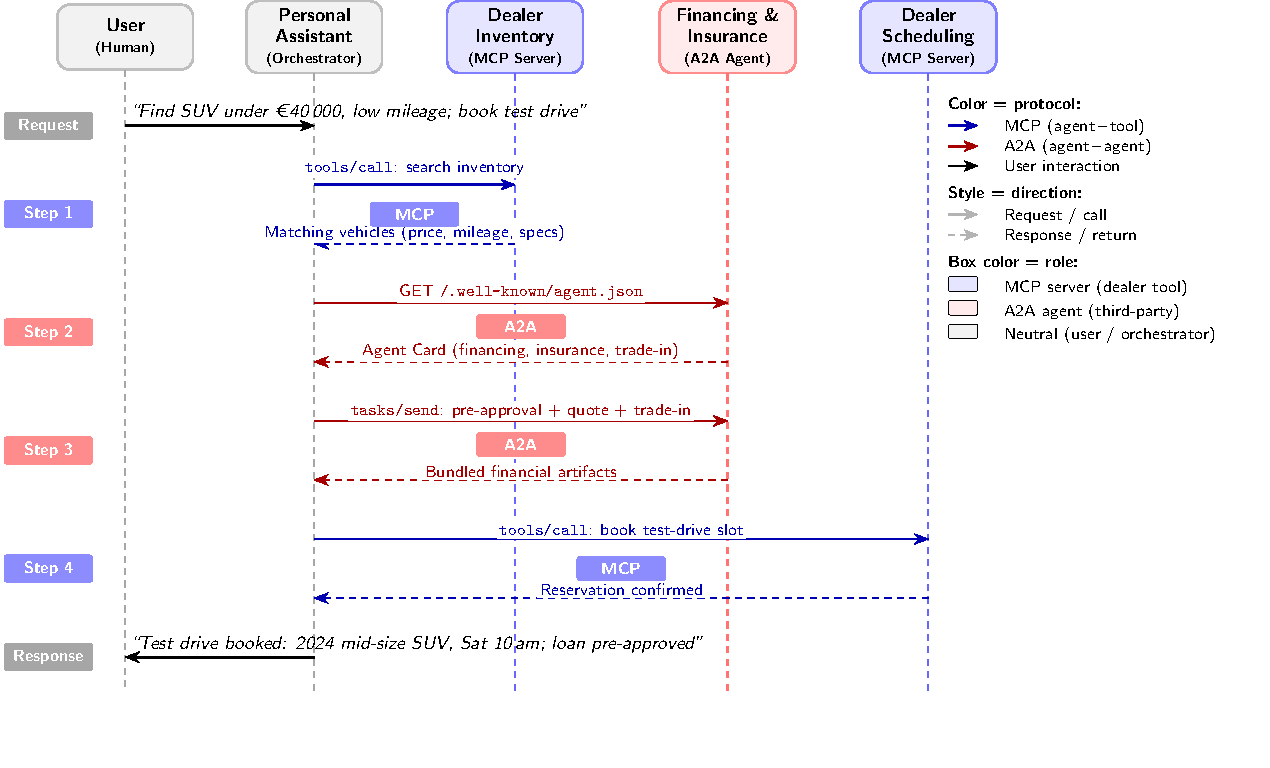
\includegraphics[width=0.88\textwidth]{fig3_sequence_car.pdf}
\caption{\textbf{Car-dealer scenario: MCP and A2A complementarity.}  The personal assistant uses MCP to invoke tools within the dealer's infrastructure (steps 1, 4: inventory search and test-drive scheduling) and A2A for cross-organizational coordination with an independent financial-services agent (steps 2--3: discovery and financing/insurance delegation).  MCP interactions occur between the orchestrating assistant and dealer-controlled MCP servers (blue arrows and boxes). A2A interactions occur between the assistant and a third-party agent (red arrows and box). Gray boxes are protocol-neutral (the human user and the orchestrating assistant, which uses both protocols). Dashed arrows indicate responses.}
\label{fig:sequence}
\end{figure*}

Both protocols have matured since their initial releases. Subsequent MCP revisions have, per the working group, addressed long-running operations, authentication, and centralized server discovery~\cite{MCP_Tasks_2025}; specific feature names and dates should be taken from the current specification rather than from this article, because the relevant sections are actively edited.

A2A has evolved in parallel, with subsequent versions reportedly addressing streaming, Agent Card expressivity, and task lifecycle~\cite{A2A_v03_2025}; we point the reader to the current specification rather than commit to a feature list that will go stale.  We also deliberately refrain from citing point-in-time adoption statistics (registry counts, organization counts, SDK availability) because such numbers change on weekly timescales and are unreliable signals of taxonomic position; the validation protocol in Section~\ref{sec:validation} instead uses reproducible, archivable adoption proxies (GitHub activity, cited deployments) tied to a snapshot date fixed in the pre-registered data-collection plan.

\subsection{The Expanding Ecosystem}\label{sec:ecosystem}

Around the MCP/A2A core, adjacent initiatives fill remaining gaps: WebMCP~\cite{WebMCP_W3C_2025} extends MCP into the browser, AG-UI~\cite{AGUI_2025} standardizes agent-to-frontend streaming, and ANP~\cite{W3C_ANP_2025} pursues DID-based decentralized discovery. New SDKs (OpenAI Agents SDK, Google ADK~v1.0, AutoGen~v0.4~\cite{Microsoft_AutoGen_2023}) treat protocol compliance as a first-class concern.  This proliferation creates coordination tensions: WebMCP and ANP handle discovery through incompatible mechanisms, AG-UI and MCP overlap in streaming, and SDK fragmentation risks undermining the consolidation that neutral stewardship was intended to achieve.  Which approaches prevail will likely be determined by \emph{de facto} adoption rather than specification completeness.

\subsection{Agent Commerce: The Missing Economic Layer}\label{sec:commerce}

The entry of payment networks into the agent space tackles what may be the WoA's oldest missing piece, because for three decades the vision lacked a credible answer to a simple question: \emph{how do agents pay for services?}

Visa's Intelligent Commerce initiative wraps existing payment rails with agent-specific authentication and tokenized credentials~\cite{Visa_TAP_2025}. Mastercard's Agent Pay targets subscription-based agent services and micro-transactions~\cite{Mastercard_AgentPay_2025}. Stripe's partnership with OpenAI integrates payment infrastructure into agent workflows~\cite{Stripe_OpenAI_ACP_2025}.

The payment initiatives intersect with new identity frameworks. Chaffer~\cite{KYA_Paradigm_2025} proposed a ``Know Your Agent'' (KYA) paradigm, analogous to KYC (Know Your Customer) in finance, requiring every transacting agent to carry verifiable credentials attesting to its identity, capabilities, operator, and liability coverage.


%%====================================================================
%% SECTION 5: EMPIRICAL VALIDATION PROTOCOL
%%====================================================================
\section{Empirical Validation Protocol}\label{sec:validation}

A taxonomy that cannot be applied by independent coders, or whose dimensions do not covary with any measurable outcome, is an organizing narrative rather than a research instrument.  We therefore treat the four-axis scheme as a testable proposal and specify three pre-registered studies.  The protocols below are registered in advance of full execution; the pilot subset (E4a) reported here demonstrates feasibility and is explicitly distinguished from confirmatory results.

\subsection{E1: Inter-Rater Reliability (feasibility check)}

\textbf{Hypothesis H1.} Given the operational codebook (Supplementary \textsection\,A1--A4), three independent coders assign the same axis value to the same system with Krippendorff's $\alpha \geq 0.70$ on all four axes.

\textbf{Corpus.} A stratified sample of 40 agent systems covering the four generations of Table~\ref{tab:taxonomy} (10 per stratum): FIPA/MAS from the AgentLink archive; Semantic-Web services from archived OWL-S directories; LLM-era frameworks and MCP servers from the public registry; post-2025-era A2A reference deployments.  The sampling frame and the 40 target identifiers are fixed before coding and included in the supplementary material so that the sample is auditable.

\textbf{Procedure.}  Three coders (PhD-level researchers in multi-agent systems, independent of the author and not involved in taxonomy design) receive the codebook, the sampling frame, and for each system (i) the canonical specification URL, (ii) one reference implementation repository.  Coders assign a value on each of the four axes together with a $\leq 50$-word evidence quote per axis.  Agreement is measured on the raw assignments, \emph{before} any consensus meeting, using Krippendorff's $\alpha$ with ordinal metric.

\textbf{Pre-registered decision rule.}  $\alpha \geq 0.70$ on all four axes supports operationality; $0.50 \leq \alpha < 0.70$ triggers codebook revision and re-coding; $\alpha < 0.50$ on any axis is reported as a negative result and that axis is flagged as not currently operationalizable.

\subsection{E2: Predictive Validity, the Axis-Coherence Hypothesis}

\textbf{Hypothesis H2.}  Across the corpus of E1, log-adoption is positively associated with axis coherence $\mathrm{coh}(S) = 1 - 2\cdot\mathrm{std}(a_1, a_2, a_3, a_4)$ after controlling for generation and application domain.

\textbf{Adoption proxies.}  A composite, pre-specified before axis values are computed, combining (a) cumulative GitHub stars and fork counts at a fixed snapshot date, (b) citations of the canonical spec in Semantic Scholar, and (c) count of independent implementations catalogued in the relevant registry.  Each component is $\log$-transformed and $z$-scored; the composite is their mean.  Proxies are collected from public sources on a fixed snapshot date, with raw queries and responses archived.

\textbf{Model.}  Linear regression $\log\text{adoption}_i = \beta_0 + \beta_c \cdot \mathrm{coh}(S_i) + \beta_g \cdot \mathbf{1}\text{[generation]} + \beta_d \cdot \mathbf{1}\text{[domain]} + \varepsilon_i$.  Pre-registered decision rule: the axis-coherence claim is supported if $\beta_c > 0$ at $p < 0.05$ with a permutation-test 95\% confidence interval excluding zero; otherwise the ``mismatch causes failure'' narrative is revised or retracted.  This is the mechanism by which the taxonomy, as a theoretical claim, is falsifiable.

\subsection{E4: LLM-as-Classifier Agreement}

\textbf{Hypothesis H3.}  The axis definitions are operational enough that a foundation model, given the codebook and system documentation, agrees with human consensus at Cohen's $\kappa \geq 0.60$.  Failure to meet this threshold is interpreted as a lack of clarity in the codebook rather than as an indictment of the model.

\textbf{Procedure.}  For each system in the E1 corpus, a frozen foundation-model release is queried with a standardized prompt containing the codebook and the same system artefacts shown to human coders.  Temperature is fixed to $0$ and three independent completions are sampled; the modal assignment per axis is retained.  Agreement with the post-consensus human labels is reported per axis.

\subsection{E4a: LLM-Self-Consistency Pilot (this paper)}\label{sec:e4a}

We ran a three-rater pilot of the LLM-as-classifier protocol against a locally archived corpus of five systems (FIPA ACL, OWL-S, LangChain, MCP, A2A).  The corpus consisted of specification snapshots fetched at a fixed date: FIPA SC00061G (Message Structure) and SC00023K (Agent Management) from the \texttt{archive.org} 2024 snapshot; OWL-S~1.2 W3C Submission; LangChain master-branch \texttt{README.md} and \texttt{AGENTS.md}; MCP specification dated 2025-03-26 (four markdown source files covering index, transport, and tools); and A2A main-branch \texttt{README.md} and \texttt{specification.md}.  Corpus files are released alongside this article (\texttt{specs/*.txt}).

Three independent rater instances were launched, each given the codebook, the same standardized prompt (\texttt{standardized\_prompt.md}), and access only to local corpus files.  Each rater was forbidden from using web tools, prior knowledge, or the other raters' outputs.  Raters were instructed to record a value $\in \{0.0, 0.5, 1.0\}$ on each axis, or \texttt{UNSPECIFIED} if the corpus was silent, and to provide a verbatim $\leq 15$-word excerpt from the corpus as evidence.  All assignments are released in \texttt{e4sim\_assignments.csv} with the evidence quotes they were supported by.

\textbf{Results.}  Pairwise percent agreement, pooled across the five systems, was $\geq 0.80$ on every axis: $\{1.00, 0.87, 0.87, 1.00\}$ for Axes~1--4 respectively.  Mean pairwise Cohen's $\kappa$, treating \texttt{UNSPECIFIED} as its own category, was $\{1.00, 0.81, 0.80, 1.00\}$, above the $\kappa \geq 0.60$ pilot threshold on every axis and above the $\kappa \geq 0.70$ target on all but the two axes where any disagreement occurred.  Only two item-level disagreements were recorded across $5\text{ systems}\times 4\text{ axes}\times 3\text{ rater pairs} = 60$ adjudications: for OWL-S on Axis~2 (R2 and R3 assigned $0.5$; R1 chose \texttt{UNSPECIFIED} because the corpus does not explicitly map OWL-S to the codebook's resource-oriented level); and for LangChain on Axis~3 (R2 and R3 assigned $1.0$ based on the \texttt{AGENTS.md} reference to chat-completion LLMs; R1 treated the evidence as insufficient and chose \texttt{UNSPECIFIED}).

All three raters independently reported that the LangChain corpus was silent on Axes~1, 2, and~4.  This is a property of the corpus we supplied (only the repository-level \texttt{AGENTS.md} and \texttt{README.md}, not the long-form docs site) and \emph{not} of the taxonomy: it shows that codebook results depend sharply on corpus composition, a property E1 must formalize.

\textbf{What this pilot does and does not show.}  It shows that when the corpus is present, three parallel LLM-rater instances applied the codebook with high self-consistency; the disagreements that did occur were confined to genuinely ambiguous evidence and were handled transparently via \texttt{UNSPECIFIED}.  It does \emph{not} substitute for E1's human inter-rater reliability: three independent LLM instances rating the same corpus can share systematic biases that $\kappa$ alone cannot detect.  It does \emph{not} test H2: a sample of five is uninformative for any regression on coherence.  Confirmatory claims require the full E1 execution with human coders and the E2 execution on 40 systems with pre-specified adoption proxies.

\subsection{Threats to Validity and Falsification Conditions}

The protocol above carries four principal threats to validity.  \emph{Construct validity}: axis values reduce a continuous design space to three ordinal levels; we mitigate by reporting sensitivity to the tie-breaking rules.  \emph{Selection bias}: the AgentLink and OWL-S archives are survivorship-biased toward documented systems; we include this bias explicitly in the limitations.  \emph{Adoption-proxy validity}: GitHub-based proxies favour open-source systems; a robustness check replaces the proxy with citation-only data.  \emph{Circularity}: the codebook was developed with reference to the same generations it classifies; E1's held-out subset (20 additional post-2025 systems not used during codebook development) tests generalization.  We pre-commit to reporting null and negative results.


%%====================================================================
%% SECTION 6: RESEARCH FRONTIER
%%====================================================================
\section{Research Frontier}\label{sec:frontier}

Progress in protocols and institutional infrastructure has made the open challenges more concrete. We organize them into four interdependent pillars: a security breach erodes trust; without trust, agents will not transact, collapsing economic models; economic misalignment invites regulatory intervention; and regulation without economic viability is unenforceable.

\textbf{Pillar 1: Security.}  The MCP/A2A stack introduces attack surfaces absent from traditional web applications: tool poisoning (malicious MCP server outputs that steer downstream reasoning), Agent Card spoofing, indirect prompt injection, and propagation of malicious behaviour through delegation chains.  The OWASP Top~10 for LLM Applications~\cite{OWASP_LLM_2025} and the International AI Safety Report~\cite{AISAFETY_2025} flag these as critical risks.  Current mitigations are partial: protocol-level authentication verifies endpoints but not tool-output integrity, and capability negotiation validates profiles but cannot detect runtime deviation.  Open problems: per-session tool sandboxing, cross-boundary anomaly detection, signed tool descriptions, and runtime integrity verification for tool outputs.

\textbf{Pillar 2: Trust, Identity, and Privacy.}  Agents can be ephemeral, created and destroyed in milliseconds, which breaks identity models built for persistent principals.  Self-Sovereign Identity (SSI) using DIDs and Verifiable Credentials, extended by the KYA paradigm~\cite{KYA_Paradigm_2025}, provides one starting point, but Sybil-resistant reputation remains unsolved.  The most pressing open problem is \emph{consent delegation}: A2A-style chains can propagate personal data across trust boundaries the user never approved (in the car-dealer scenario, the user authorized an inventory search, not financial disclosure to a third party).  Key directions: federated reputation, privacy-preserving authentication via zero-knowledge proofs, consent-propagation protocols in task metadata, and formal models of multi-hop authorization.

\textbf{Pillar 3: Economics.}  Multi-agent workflows accumulate unpredictable micro-costs, and without reliable quality signals the WoA risks a ``market for lemons'' collapse.  Commercial rails have begun to emerge, but stable incentive structures and cost-transparency mechanisms have yet to materialize.

\textbf{Pillar 4: Governance.}  The EU AI Act~\cite{EUAI_2024} mandates human oversight of high-risk AI systems, a requirement that strains when no single human monitors a multi-hop delegation chain.  Cross-jurisdictional workflows compound the problem, as delegation chains may span conflicting regulatory regimes with no reconciliation mechanism.  Open gaps: agent liability models (vicarious vs.\ product liability) and automated compliance auditing.

\textbf{Cross-cutting: Evaluation.}  Benchmarks such as AgentBench and ProtocolBench provide initial frameworks, but comprehensive multi-agent testing remains an open challenge; the validation protocol of Section~\ref{sec:validation} is complementary to these benchmarks but addresses taxonomic applicability rather than task performance.


%%====================================================================
%% SECTION 7: CONCLUSION
%%====================================================================
\section{Conclusion}\label{sec:conclusion}

We have reformulated the ``paradigm shift'' narrative about the Web of Agents as a classificatory proposal with (i) a four-axis functional taxonomy, (ii) an operational codebook that makes the axes applicable by third parties, and (iii) a pre-registered three-part validation protocol together with a five-system self-consistency pilot.  Under this framing the axis-coherence hypothesis, that adoption is associated with alignment across axes rather than with any single axis value, is the testable form of the claim that prior generations failed from internal mismatches.  The pilot already surfaces a candidate counter-example (a low-coherence profile coexisting with strong adoption), and we have pre-committed to reporting the full E1/E2/E4 results, including null findings, without post-hoc rescue.  If the axis-coherence effect is null, the taxonomy remains useful as an organising instrument but loses its explanatory ambition.  If the effect holds, the research frontier (Section~\ref{sec:frontier}) gains a concrete design principle: cross-axis alignment is a property to engineer for, not only to observe.


%%====================================================================
%% BIBLIOGRAPHY
%%====================================================================
\bibliographystyle{plainnat}
\bibliography{references}

\end{document}
